\subsubsection{Output power}
\label{sec:eval:pumpspot:pwr}

In order to learn
about the scaling behavior
of the output power,
we look 
at the light-light characteristics
obtained from different
pump spot sizes.
Output scaling with area
only works up to a point,
above which
amplified spontaneous emission (ASE) losses
become significant
\cite{Hessenius2011}.
Bedford et al. \cite{Bedford2005}
also estimate
there to be
a critical diameter
above which lateral lasing
is likely to occur
before the intended
transversal lasing.
With our measurements,
we're interested
to see the experimental
scaling behavior
of our structure
for spot sizes
realistic in real world applications.

\begin{figure}
\centering
\subfigure{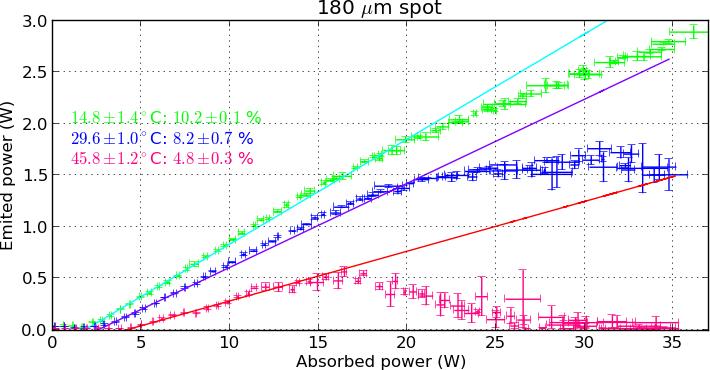
\includegraphics[width=14.5cm]{img/LL_spot180um.png}}
\subfigure{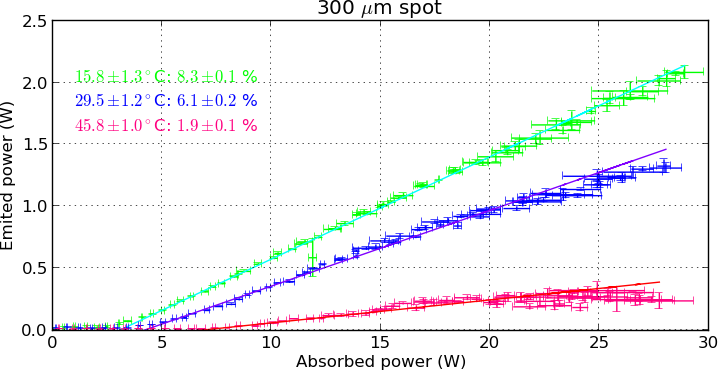
\includegraphics[width=14.5cm]{img/LL_spot300um.png}}
\subfigure{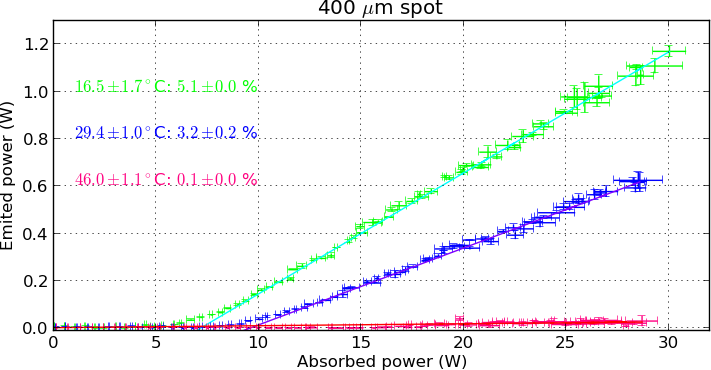
\includegraphics[width=14.5cm]{img/LL_spot400um.png}}
\caption{Light-light characteristics
for different spot sizes
obtained with spherical lenses.
The efficiency decreases
for increased spot size.
This may be due to
inefficient heat extraction
manifested in sub-area scaling of $\Rth$,
discussed in section~\ref{sec:eval:pumpspot:rth}.}
\label{img:LL_spot_scaling}
\end{figure}

Figure~\ref{img:LL_spot_scaling}
plots the resulted
light-light characteristics
for various spot sizes,
measured at the heat sink temperatures
$\{15,30,45\}\,^\circ\mathrm{C}$,
using spherical lenses
for both $\mathrm{L}_\mathrm{p1}$ and $\mathrm{L}_\mathrm{p2}$.
The average maintained heat sink temperature,
plus-minus its standard deviation,
is stated in each of the subplots,
accompanied by the slope efficiency
corresponding to
the straight lines.
The slope efficiency
is obtained
by taking into account
only the data points
of the linear segment.
The onset of
the roll over region
is ignored.

The most obvious conclusion
we can draw from these measurements
is that
our device is not power scalable:
the conversion efficiency
decreases for larger pump spots,
while in a scalable device
it should not.
Consequentially,
the maximally achieved
output power
is not increased
for larger pump spots.
In order to explain this
we acknowledge that
with larger pump spots
we're more likely
to hit non-radiative defects
\cite{Korpi2010}.
Secondly,
the thermal resistance
is empirically demonstrated
to decrease less efficiently
than with irradiated area.
The initial explanation
why VECSELs are expected
to power scale
relies on the one dimensional
heat extraction.
In reality
the contribution
of lateral cooling
must not be neglected
\cite{Chernikov2011}.

Beside the decrease
in conversion efficiency,
the roll over point
shifts to higher absorbed power
for larger pump spots.
This indicates
the structure
to heat up less
for larger pump spots.
The findings
concerning the thermal resistance
discussed in \ref{sec:eval:pumpspot:rth}
support this interpretation.

I performed
these scaling measurements
also with lens
$\mathrm{L}_\mathrm{p1}$
replaced by
an achromatic lens.
We would not assume
to find significant
differences
in the scaling behavior
since the spectral profile
of our pump source
is fairly narrow,
Fig.~\ref{img:pumpspectrum}.
Nevertheless,
this assumption needs to be tested.
Secondly,
these measurements yield
additional data points
for the thermal resistance
scaling behavior,
discussed in \ref{sec:eval:pumpspot:rth}.

The investigated spot diameters
are $\{222,333,444\}\,\mu\mathrm{m}$
for the achromatic configuration.
The used output coupler
is not optimal
for spot sizes larger than
$400\,\mu\mathrm{m}$.
The performance
corresponding to
the $444\,\mu\mathrm{m}$ spot
was indeed worse
than the one 
corresponding to
the $333\,\mu\mathrm{m}$ spot.
However,
the $222\,\mu\mathrm{m}$ spot
performed even worse.
Given this discrepancy,
I have to discard
the results
from the spot scaling experiments
in the achromatic setting.
Non the less,
all of these three measurements
showed an improved performance
with respect to
the spherical lens configuration.

We don't know the exact beam shape,
and the estimation
of the spot size
is the result
of a ray optical consideration.
The uncertainty
resulting from this approach
should be looked into more closely
in future investigations.
The fact that the pump beam shape
is relevant
was demonstrated
in \cite{Chernikov2010}.
The improved output performance
seen in our setup,
by simply changing
the type of
one of the pump delivery lenses,
also indicate
on the importance
of the pump profile.
A summary on beam shape alteration
is given
in appendix~\ref{app:spatial}
and \cite{Mansell2000}. 

For now we can only speculate
why incorporating
the achromatic lens
improves the output performance
the way it did.
I investigated
the $333\,\mu\mathrm{m}$ configuration
more thoroughly.
The results were
reproducible and thus credible.
The measurements
concerning the proposed improvements
\cite{Hader2011}
presented in section~\ref{sec:eval:maxout},
were obtained in this configuration.